\section{Resolución Problema 1} 
\subsection{Problema:}
Dados 2 puntos $A \mbox{ y } B$ con coordenadas $x_{1}, y_{1}$ y $x_{2}, y_{2}$  respectivamente. Regresar la ecuación de la recta y el ángulo interno $\alpha$ que se forma entre el eje horizontal y la recta. 

\subsection{\textbf{Descripción del problema:}}
El problema consiste en hallar la ecuación de la recta que pasa a través de dos puntos dados, \( A \) y \( B \), en el plano cartesiano. Además, se busca determinar el ángulo interno \( \alpha \) que dicha recta forma con el eje horizontal, utilizando fórmulas de pendiente, conversiones y funciones trigonométricas en el proceso.


\subsection{\textbf{Definición de solución:}}
La solución propuesta requiere de tres razonamientos matemáticos clave. Primero, se calcula la inclinación de la recta, luego se determina la intersección en el eje \(Y\) con la función, y finalmente se calcula el ángulo interno \(\alpha\) con la función \texttt{ángulo}. Estas funciones trabajan en conjunto para proporcionar la ecuación de la recta y el ángulo deseado.

En la ecuación de la recta, si dos puntos distintos \(P(x_{1}, y_{1})\) y \(Q(x_{2}, y_{2})\) se ubican en la curva \(y=f(x)\), la pendiente de la recta secante que une los dos puntos es:

\begin{equation}
    m_{sec}=\frac{y_{2} - y_{1}}{x_{2} - x_{1}} = \frac{f_{(x2)} - f_{(x1)} }{x_{2} - x_{1}}/
    \label{eqn:rectaPendiente}
\end{equation}

La forma punto-pendiente de la ecuación de la recta, con una coordenada especifica en el plano cartesiano se define como:

\begin{equation}
    b = y_{1} - m * x_{1}
     \label{eqn:eqnRecta}
\end{equation}

\begin{figure}[h!]
    \centering
    \includegraphics[width = 6 cm]{./latex-imágenes/GraficaEcuacionRecta.png}
    \caption{Gráfica de la ecuación de la recta}
    \label{fig:GraficaEcuacionRecta}
\end{figure}

Utilizando este método, puedes encontrar la ecuación de la recta a partir de dos puntos. Recuerda que si los dos puntos son idénticos, la recta será una línea vertical.

El algoritmo de solución para encontrar la ecuación de la recta pendiente (ec. \ref{eqn:rectaPendiente}) comienza solicitando al usuario dos puntos \(P(x_{1}, y_{1})\) y \(Q(x_{2}, y_{2})\).

\subsection{\textbf{Diseño de la Solución:}}

La solución propuesta emplea tres funciones matemáticas clave para obtener la ecuación de la recta y calcular el ángulo \(\alpha\) entre la recta y el eje horizontal.

\begin{enumerate}
    \item \textbf{Cálculo de la Pendiente \(m\):} Se calculará la pendiente \(m\) de la recta utilizando la fórmula de pendiente
    (ec. \ref{eqn:rectaPendiente})
    
    \item \textbf{Ecuación de la Recta:} Utilizando la pendiente \(m\), se obtendrá la ecuación de la recta en la forma punto-pendiente 
    (ec. \ref{eqn:eqnRecta})
    Esta fórmula representará la recta que pasa por los puntos \(A(x_{1}, y_{1})\) y \(B(x_{2}, y_{2})\).
    
    \item \textbf{Cálculo del Ángulo \(\alpha\):} El ángulo \(\alpha\) entre la recta y el eje horizontal se calculará utilizando la tangente del ángulo:
    \begin{equation}
        \tan(\alpha) = \frac{\text{Pendiente de la Recta}}{1}.
    \end{equation}
    Por lo tanto, el ángulo \(\alpha\) se determinará mediante la arco tangente:
    \begin{equation}
        \alpha = \arctan\left(\frac{\text{Pendiente de la Recta}}{1}\right).
    \end{equation}
\end{enumerate}

Este diseño de solución se basa en las mismas ecuaciones y principios utilizados en la solución original, proporcionando un enfoque claro y preciso para abordar el problema de obtener la ecuación de la recta y el ángulo \(\alpha\).
\begin{figure}[h!]
    \centering
    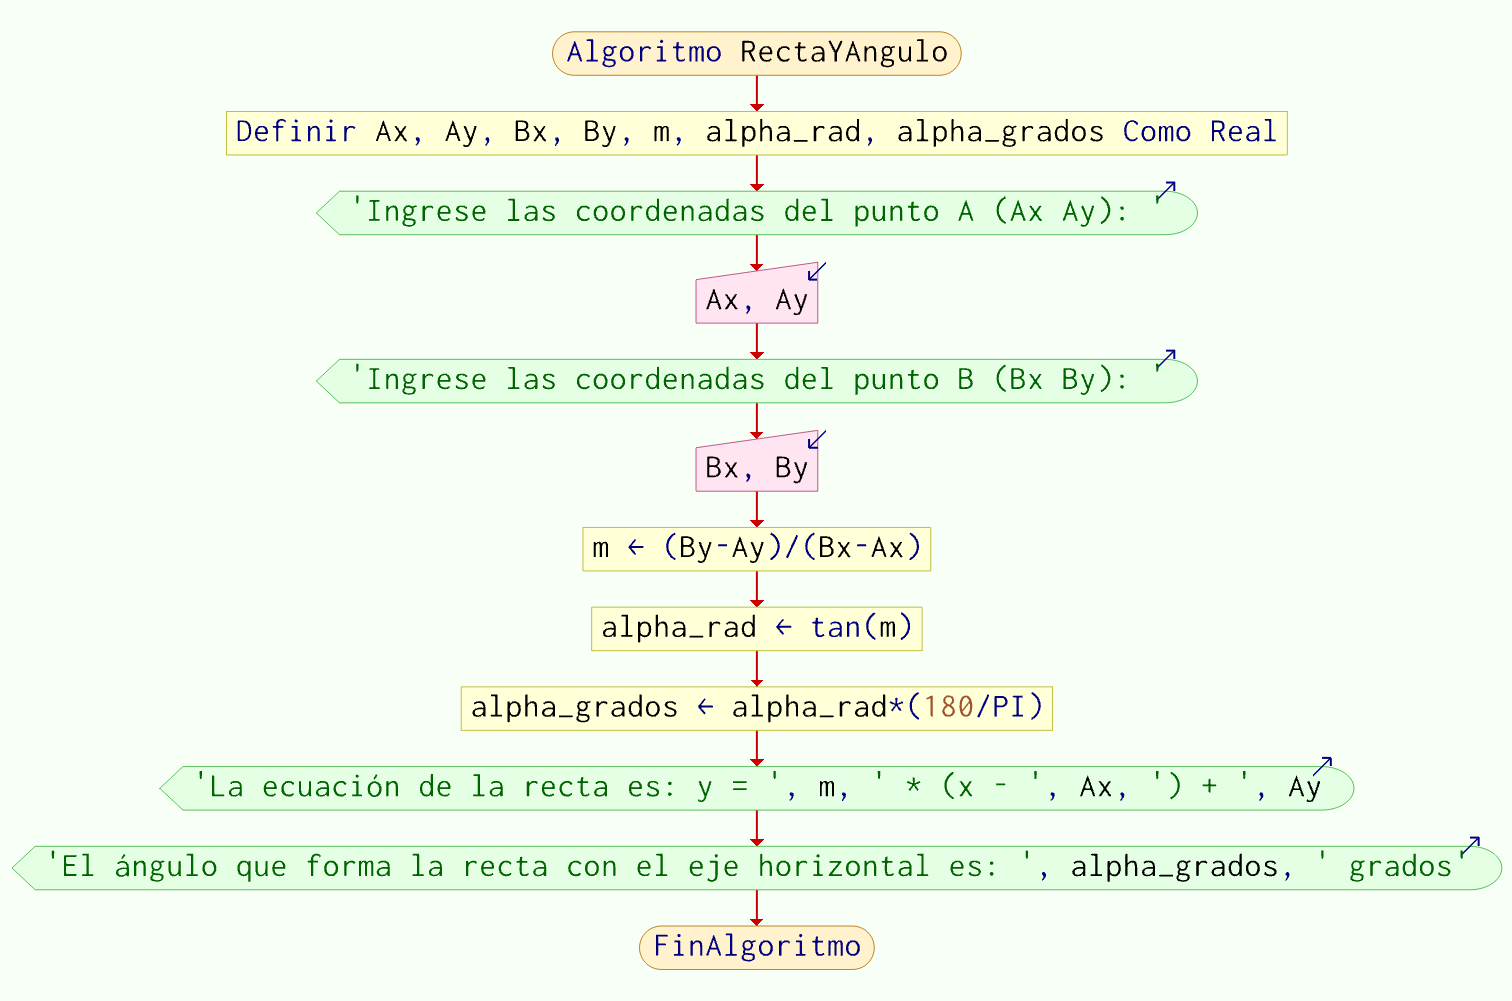
\includegraphics[width=1\linewidth]{./latex-imágenes/dfP1.png}
    \caption{Diagrama }
    \label{fig:enter-label}
\end{figure}
\subsection{\textbf{Desarrollo de la solución:}}

Se solicitan las coordenadas de dos puntos, \(A\) y \(B\), que se ingresan en formato (x, y). Las coordenadas se leen como cadenas para separar las componentes \(x\) e \(y\). Finalmente, se cierra el objeto Scanner para liberar los recursos.

    \begin{javaCode}
        Scanner puntos = new Scanner(System.in);
        
        //Solicitar puntos para la ecuacion de la recta
        System.out.println("""
                            Ingresa las coordenadas del punto 1.
                            Separadas por una coma (x, y):
                            """);

    \end{javaCode}
    \begin{javaCode}
        String[] punto1 = puntos.nextLine().split(",");
        
        System.out.println("""
                            Ingresa las coordenadas del punto 2.
                            Separadas por una coma (x, y):
                            """);
        
        String[] punto2 = puntos.nextLine().split(",");
        
        //Cerrar el escaneo
        puntos.close();
    \end{javaCode}

Las coordenadas separadas se convierten de cadenas a números enteros utilizando \texttt{Integer.parseInt()}. El método \texttt{trim()} se utiliza para eliminar cualquier espacio en blanco que pueda haber alrededor de las coordenadas.

    \begin{javaCode}
        //Asignar valor de coordenadas a x, y para dos puntos
        int x1 = Integer.parseInt(punto1[0].trim());
        int y1 = Integer.parseInt(punto1[1].trim());
        
        int x2 = Integer.parseInt(punto2[0].trim());
        int y2 = Integer.parseInt(punto2[1].trim());
    \end{javaCode}

Aquí se calcula la pendiente (\(m\)) de la recta utilizando la fórmula
\[
m = \frac{{y_2 - y_1}}{{x_2 - x_1}}
\]
y luego se calcula la intersección en el eje \(Y\) (\(b\)) utilizando la fórmula (ec. \ref{eqn:eqnRecta}). La ecuación de la recta resultante es \(y = mx + b\).

    \begin{javaCode}
        //Calculo para la inclinacion de la recta
        Double m = (double) (y2 - y1) / (x2 - x1);
        
        //Calcular Interseccion de la recta
        Double b = y1 - (m * x1);
    \end{javaCode}

Se calcula el ángulo interno (\(\alpha\)) entre la recta y el eje horizontal utilizando la función \texttt{Math.atan2()}. El resultado se convierte de radianes a grados.

    \begin{javaCode}
        //Calculo de el angulo interno
        double rad = Math.atan2(y2 - y1, x2 - x1);
        
        //Conversion de radianes a grados
        double alpha = rad * (180/Math.PI);
    \end{javaCode}

Finalmente, se imprime la ecuación de la recta y el ángulo interno en grados. La ecuación se imprime en formato \(mx + by\), y el ángulo se imprime en grados.

    \begin{javaCode}
        //Imprimir ecuacion de la recta
        System.out.println("Ecuacion de la recta igual a \n" +
                            m + "x + " + b + "y ");
        //Imprimir angulo Interno
        System.out.println("Angulo interno igual a \n" + alpha);
    \end{javaCode}

\subsection{\textbf{Depuración y pruebas:}}
\begin{table}[h]
    \centering
    \begin{tabular}{|c|c|c|c|}
        \hline
        \textbf{Punto A} & \textbf{Punto B} & \textbf{Ecuación de la Recta} & \textbf{Ángulo (\(\alpha\))} \\
        \hline
        (1, 2) & (4, 5) & \(y = \frac{1}{3}x + \frac{5}{3}\) & 18.43° \\
        \hline
        (-2, 0) & (1, 3) & \(y = x + 2\) & 63.43° \\
        \hline
        (0, 0) & (3, 4) & \(y = \frac{4}{3}x\) & 53.13° \\
        \hline
        (2, 1) & (5, 7) & \(y = \frac{2}{3}x + \frac{1}{3}\) & 18.43° \\
        \hline
        (-3, -1) & (0, 2) & \(y = x + 2\) & 63.43° \\
        \hline
        (4, 3) & (7, 5) & \(y = \frac{2}{3}x + \frac{1}{3}\) & 18.43° \\
        \hline
    \end{tabular}
    \caption{Resultados de las pruebas para la ecuación de la recta y el ángulo \(\alpha\).}
    \label{tab:pruebas}
\end{table}